\chapter{approaching logo process}
\label{sec:tempest_logo}
\lhead[tempest]{}
\lstset{style=6502Style}

\begin{figure}[H]
    \centering
    \begin{adjustbox}{width=11cm,center}
      
\includegraphics[width=12cm]{src/titles/title.png}%
    \end{adjustbox}
  \caption{The Tempest Title Rainbow.}
\end{figure}

The \textit{TEMPEST} title sequence is a thing of simple beauty. It cascades towards
us from afar in a rainbow of shifting colours. It is a glimpse into the future of video
games, where the illusion of three dimensions will become commonplace. Despite its rawness,
and even its crudity, it beguiles us into accepting Tempest's world of near infinite depth.
A world in which things that are so far away they are almost invisible quickly come up on us
from the deep.

To understand how it was achieved we must start with the bare building blocks. The routines that
get the letters onto the screen. There are five individual letters in Tempest, and we have a routine
for each.

\clearpage
\begin{minipage}[c]{0.48\linewidth}
\begin{figure}[H]
    \centering
    \begin{adjustbox}{width=4cm,center}
      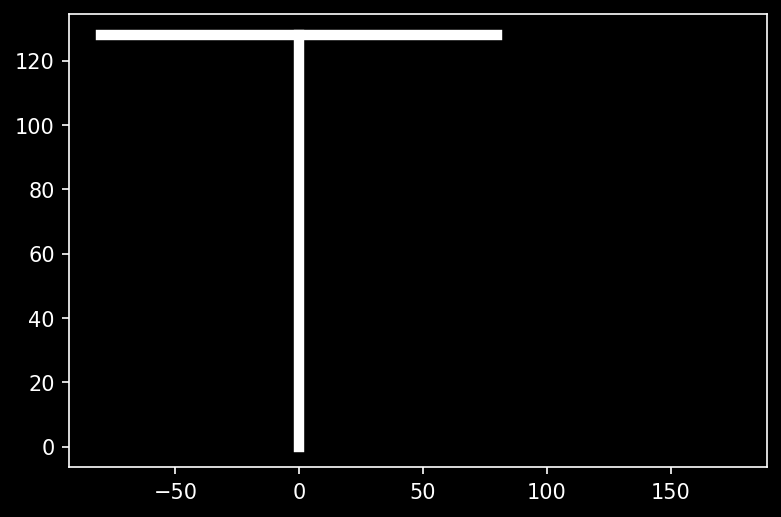
\includegraphics[width=12cm]{src/titles/letters/T.png}%
    \end{adjustbox}
\end{figure}
\end{minipage}
\begin{minipage}[c]{0.48\linewidth}
\begin{lstlisting}[basicstyle=\scriptsize\ttfamily]
T:      VCTR 0,80,CB            ;T
        VCTR -50,0,0
        VCTR 0A0,0,CB
\end{lstlisting}
\vspace*{\fill}
\end{minipage}

\begin{minipage}[c]{0.48\linewidth}
\begin{figure}[H]
    \centering
    \begin{adjustbox}{width=4cm,center}
      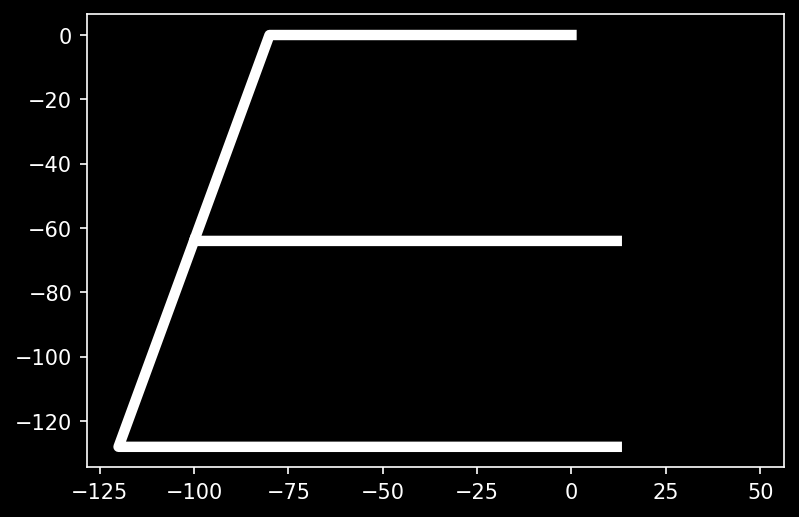
\includegraphics[width=12cm]{src/titles/letters/E.png}%
    \end{adjustbox}
\end{figure}
\end{minipage}
\begin{minipage}[c]{0.48\linewidth}
\begin{lstlisting}[basicstyle=\scriptsize\ttfamily]
E:      VCTR -50,0,CB           ;E
        VCTR -14,-40,CB
        VCTR 70,0,CB
        VCTR -70,0,0
        VCTR -14,-40,CB
        VCTR 84,0,CB
\end{lstlisting}
\vspace*{\fill}
\end{minipage}

\begin{minipage}[c]{0.48\linewidth}
\begin{figure}[H]
    \centering
    \begin{adjustbox}{width=4cm,center}
      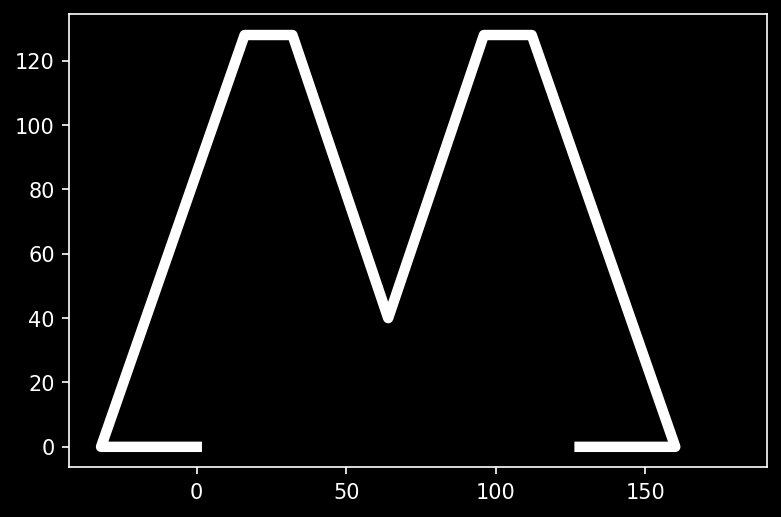
\includegraphics[width=12cm]{src/titles/letters/M.png}%
    \end{adjustbox}
\end{figure}
\end{minipage}
\begin{minipage}[c]{0.48\linewidth}
\begin{lstlisting}[basicstyle=\scriptsize\ttfamily]
M:      VCTR -20,0,CB           ;M
        VCTR 30,80,CB
        VCTR 10,0,CB
        VCTR 20,-58,CB
        VCTR 20,58,CB
        VCTR 10,0,CB
        VCTR 30,-80,CB
        VCTR -20,0,CB
        RTSL
\end{lstlisting}
\vspace*{\fill}
\end{minipage}

\begin{minipage}[c]{0.48\linewidth}
\begin{figure}[H]
    \centering
    \begin{adjustbox}{width=4cm,center}
      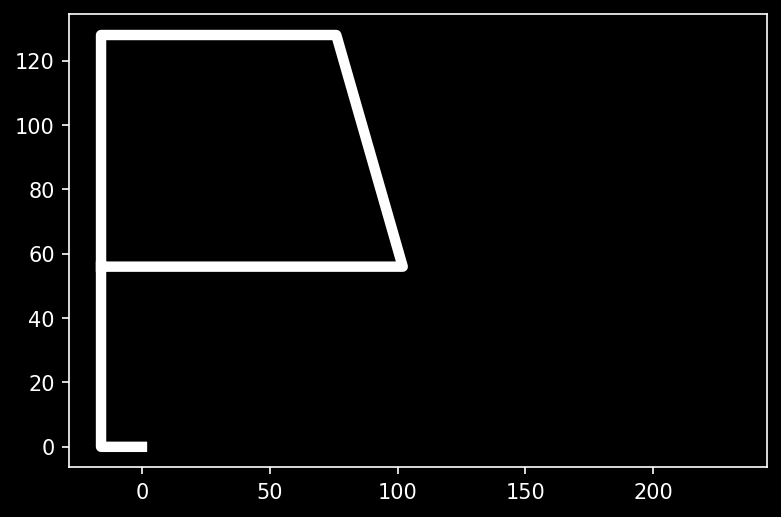
\includegraphics[width=12cm]{src/titles/letters/P.png}%
    \end{adjustbox}
\end{figure}
\end{minipage}
\begin{minipage}[c]{0.48\linewidth}
\begin{lstlisting}[basicstyle=\scriptsize\ttfamily]
P:      VCTR -10,0,CB           ;P
        VCTR 0,80,CB
        VCTR 5C,0,CB
        VCTR 1A,-48,CB
        VCTR -76,0,CB
        RTSL
\end{lstlisting}
\vspace*{\fill}
\end{minipage}

\begin{minipage}[c]{0.48\linewidth}
\begin{figure}[H]
    \centering
    \begin{adjustbox}{width=4cm,center}
      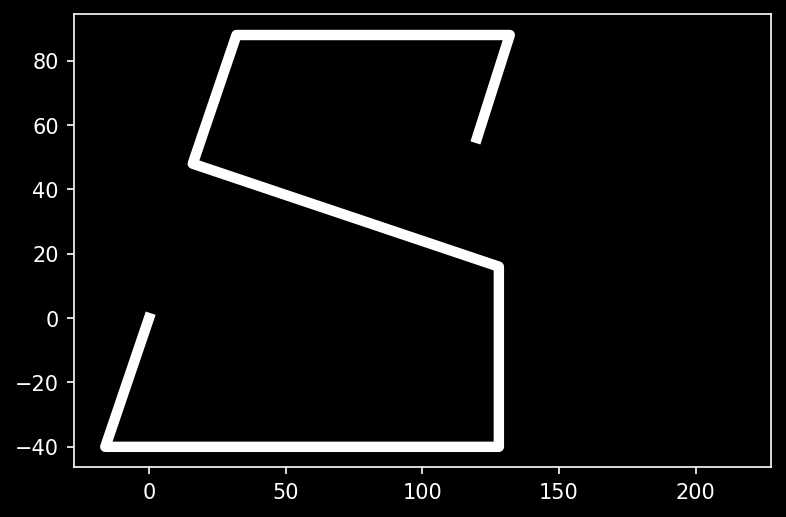
\includegraphics[width=12cm]{src/titles/letters/S.png}%
    \end{adjustbox}
\end{figure}
\end{minipage}
\begin{minipage}[c]{0.48\linewidth}
\begin{lstlisting}[basicstyle=\scriptsize\ttfamily]
S:      VCTR -10,-28,CB         ;S
        VCTR 90,0,CB
        VCTR 0,38,CB
        VCTR -70,20,CB
        VCTR 10,28,CB
        VCTR 64,0,CB
        VCTR -0C,-20,CB
        RTSL
\end{lstlisting}
\vspace*{\fill}
\end{minipage}

\clearpage
If you look closely you can see each letter is a routine in its own right. Each consists of the vector commands
we encountered in
\hyperref[sec:cursors]{\textcolor{blue}{'cursors'}}
and
\hyperref[sec:wells]{\textcolor{blue}{'wells'}}. Each concludes with an \icode{RTSL} statement that returns
from the routine. This mean that in order to build the \textit{TEMPEST} title image
we can create a routine called \icode{VORLIT} that writes it out in full.
\begin{minipage}[c]{0.58\linewidth}
\begin{figure}[H]
    \centering
    \begin{adjustbox}{width=6cm,center}
      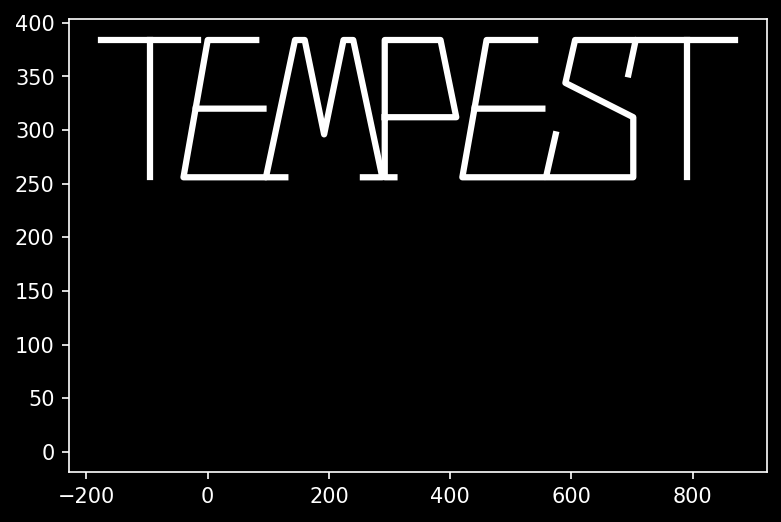
\includegraphics[width=12cm]{src/titles/letters/TEMPEST.png}%
    \end{adjustbox}
\end{figure}
\end{minipage}
\begin{minipage}[c]{0.38\linewidth}
\begin{lstlisting}[basicstyle=\scriptsize\ttfamily]
VORLIT:
        CNTR
        VCTR -1B0,100,0
        JSRL T
        VCTR 60,0,0
        JSRL E
        VCTR 24,0,0
        JSRL M
        VCTR 34,0,0
        JSRL P
        VCTR 0F8,48,0
        JSRL E
        VCTR 16,28,0
        JSRL S
        VCTR 60,-60,0
        JMPL T
\end{lstlisting}
\vspace*{\fill}
\end{minipage}

Equipped with \icode{VORLIT} as a shorthand for drawing the \icode{TEMPEST} title logo onto the
screen we can use two other Vector Drawing instructions to alter the scale of the logo and colour
of the logo when we draw it. If we adjust the scale and the colour as we go along we can create the
effect of a cascading series of differently coloured titles receding into the distance. 

Fortunately there are vector commands that will allow us to do all of this. Each command is a two-byte
Op Code. There's one for setting the color to be used when drawing, one for setting the scale to use
when drawing (allowing us to make the title big or small), and one for calling our \icode{VORLIT}
routine to actually draw the title logo in our selected colour and scale.

\begin{figure}[H]
  {
    \setlength{\tabcolsep}{3.0pt}
    \setlength\cmidrulewidth{\heavyrulewidth} % Make cmidrule = 
    \begin{adjustbox}{width=12cm,center}

      \begin{tabular}{lll}
        \toprule
    OpCode Description    &     OpCode      &  How We Use It.\\
        \midrule
    New color/intensity   &     0x6000   &  \icode{000} will give the color and intensity.\\
    New scale             &     0x7000   &  \icode{000} will give the scale to draw at.\\
    Jump to subroutine    &     0xA000   &  \icode{000} can be populated with an address, e.g. \icode{VORLIT}. \\
      \end{tabular}
    \end{adjustbox}
  }
\end{figure}

So we can imagine issuing a series of three vector commands such as the ones given below to draw our
logo.
\begin{figure}[H]
  {
    \setlength{\tabcolsep}{3.0pt}
    \setlength\cmidrulewidth{\heavyrulewidth} % Make cmidrule = 
    \begin{adjustbox}{center}
      \begin{tabular}[t]{lll}
        \toprule
        Op Code & Parsed Data & Written to Screen\\

        \midrule
          \icode{7220}
        &
        \makecell[tl]{
          \begingroup
          \renewcommand{\arraystretch}{.8} % Default value: 1
          \begin{tabular}[t]{ll}
            Set Scale: & \icode{220}\\
            \icode{} &  \\
          \end{tabular}
          \endgroup
        } &
        \multirow{3}{*}[-0.1cm]{
          \makecell[tl]{
            
\includegraphics[height=2.3cm]{titles/rainbow/0.png}%
          }
        } \\
        \addlinespace
          \icode{6800}
        &
        \makecell[tl]{
          \begingroup
          \renewcommand{\arraystretch}{.8} % Default value: 1
          \begin{tabular}[t]{ll}
            New Color: & White\\
            Intensity: &  \icode{00}\\
          \end{tabular}
          \endgroup
        } &
        \\
        \addlinespace
          \icode{AFA7}
        &
        \makecell[tl]{
          \begingroup
          \renewcommand{\arraystretch}{.8} % Default value: 1
          \begin{tabular}[t]{ll}
            Jump to Routine: & \icode{VORLIT}  \\
            \icode{} &  \\
          \end{tabular}
          \endgroup
        } &
        \\

        \bottomrule
      \end{tabular}
    \end{adjustbox}
  }
\end{figure}

If we repeat these commands, changing the color and reducing the scale as we go, we 
should expect to achieve the effect we're looking for. And this is exactly what we find
in \icode{SCARNG}. This routine builds the title rainbow by adding the three commands above
to the vector list and it does this 19 times, adjusting the color and reducing the scale
as it goes.
\begin{lstlisting}
        .SBTTL  LOGO RAINBOW BUILDER
SCARNG:
    ; DRAW THE TEMPEST TITLE RAINBOW. THIS CONSISTS OF 19 ITERATIONS
    ; OF THE TITLE IMAGE IN EVER INCREASING DEPTH AND VARYING COLORS.
    ; A - CONTAINS THE LOW BYTE OF THE ADDRESS FOR VORLIT.
    ; X - CONTAINS THE HI  BYTE OF THE ADDRESS FOR VORLIT.
    STA PYL            ; STORE LOW BYTE OF VORLIT IN PYL
    STX PXL            ; STORE HI  BYTE OF VORLIT IN PYL
    LDA NEARY          ; PUT THE NEAREST ALLOWED POSITION IN A
    STA INDEX1         ; STORE IT IN INDEX1
    
    ; THIS IS THE LOOP THAT DRAWS THE TITLE RAINBOW, ONE TITLE
    ; AT A TIME, UNTIL WE REACH THE FURTHEST ALLOWED POSITION.
    ; WITH THE NEAREST POSITION STORED IN INDEX1 WE INCREMENT
    ; IT AT EACH ITERATION TO DRAW THE NEXT TITLE A LITTLE
    ; FURTHER AWAY UNTIL IT EQUALS FARY.
    BEGIN                          ; START OF THE LOOP
    
    ; FIRST WE SET THE SCALE OF THE TITLE IMAGE TO DRAW IN THIS
    ; ITERATION. THIS WILL DETERMINE HOW FAR AWAY IT SEEMS. TO DO
    ; THIS WE BASE IT ON THE DISTANCE VALUE IN INDEX1 AND CALL
    ; VGSCAL TO ADD A VECTOR COMMAND THAT SETS THE SCALE WE WILL
    ; DRAW THE TITLE AT. WE SET TWO SCALE TYPES, LINEAR AND BINARY.
    ; LINEAR SCALE FACTOR (0=FULL SIZE, FF=1/256 SIZE, FE=2/256, ETC.)
    ; BINARY SCALE FACTOR (0=FULL SIZE,1=1/2 SIZE, ETC.)
    LDA INDEX1         ; GET THE CURRENT DISTANCE VALUE.
    ASL                ; SHIFT LEFT ONE BIT (I.E. MULTIPLY BY 2).
    ASL                ; MULTIPLY BY 2 AGAIN.
    AND I,7F           ; AND WITH 7F TO GET OUR SCALE VALUE.
    TAY                ; SET RESULT AS OUR LINEAR SCALE VALUE.
    LDA INDEX1         ; GET THE CURRENT DISTANCE VALUE.
    LSR                ; DIVIDE BY 32 BY SHIFTING RIGHT FIVE TIMES.
    LSR                ; TWO TIMES.
    LSR                ; THREE TIMES.
    LSR                ; FOUR TIMES.
    LSR                ; FIVE TIMES.
    JSR VGSCAL         ; ADD THE COMMAND SETTING BINARY AND LINEAR SCALE.
    
    ; NEXT WE SET THE COLOR WE WILL DRAW THE TITLE WITH. WE USE THE
    ; CURRENT DISTANCE TO CHOOSE THIS COLOR AND 'SET' IT BY CALLING
    ; VGSTAT. WE TURN THE DISTANCE INTO A COLOR BY SHIFTING IT RIGHT
    ; THREE BITS - THIS GIVES US A COLOUR VALUE THAT VGSTAT CAN USE.
    LDA INDEX1         ; GET THE CURRENT DISTANCE VALUE.
    CMP NEARY          ; IS IT EQUAL TO THE NEAREST POINT (I.E. THE TOP)?
    IFEQ               ; IF SO..
    LDA I,WHITE        ; .. PAINT IT WHITE.
    ELSE               ; OTHERWISE..
    LSR                ; DIVIDE BY 8 BY SHIFTING LEFT THREE TIMES.
    LSR                ; TWO TIMES.
    LSR                ; THREE TIMES.
    NOP                ; A NO-OP.
    AND I,7            ; MAKE THE RESULT BETWEEN 0 AND 7
    CMP I,7            ; IS IT EQUAL TO 7 (I.E. BLACK)?
    IFEQ               ; IF SO..
    LDA I,RED          ; USE RED FOR BLACK
    ENDIF
    ENDIF
    TAY                ; STORE THE COLOR IN Y
    LDA I,68           ; SET THE COMMAND BITS FOR VGSTAT
    JSR VGSTAT         ; SET COLOR BY CALLING VGSTAT
    
    ; NOW WE'RE READY TO PAINT THE TITLE. REMEMBER WE STORED THE ADDRESS
    ; TO VORLIT IN PYL AND PXL. SO VGJSRL WILL USE THAT TO DRAW THE VECTORS
    ; CONTAINING THE TEMPEST TITLE IN THE VORLIT ROUTINE.
    LDA PYL            ; LOAD THE LOW BYTE OF VORLIT TO A.
    LDX PXL            ; LOAD THE HI  BYTE OF VORLIT TO A.
    JSR VGJSRL         ; DRAW THE TEMPEST TITLE.
    
    ; NOW GET READY TO DRAW THE NEXT ITERATION. WE INCREMENT INDEX1
    ; BY 2 AND DRAW ANOTHER TITLE FURTHER AWAY, UNTIL WE REACH THE FARTHEST
    ; ALLOWED DISTANCE (FARY).
    LDA INDEX1         ; GET THE CURRENT DISTANCE VALUE.
    CLC                ; CLEAR THE CARRY SO ADDING WILL HAPPEN OK.
    ADC I,2            ; ADD 2 TO THE CURRENT DISTANCE.
    STA INDEX1         ; AND STORE IT IN INDEX1.
    CMP FARY           ; IF IT IS EQUAL TO FARY, EXIT..
    CSEND              ; OTHERWISE LOOP AND DRAW ANOTHER TITLE.
\end{lstlisting}

We can see how the commands mutate and slowly build up the rainbow piece by piece
for all 19 iterations in the table that follows.
\begin{figure}[H]
  {
    \setlength{\tabcolsep}{3.0pt}
    \setlength\cmidrulewidth{\heavyrulewidth} % Make cmidrule = 
    \begin{adjustbox}{center}
      \begin{tabular}[t]{lll}
        \toprule
        Vector Commands & Command Meaning & Result on Screen\\

        \midrule
          \icode{7228}
        &
        \makecell[tl]{
          \begingroup
          \renewcommand{\arraystretch}{.8} % Default value: 1
          \begin{tabular}[t]{ll}
            Set Scale: & \icode{228}\\
            \icode{} &  \\
          \end{tabular}
          \endgroup
        } &
        \multirow{3}{*}[-0.1cm]{
          \makecell[tl]{
            
\includegraphics[height=2.3cm]{titles/rainbow/1.png}%
          }
        } \\
        \addlinespace
          \icode{6801}
        &
        \makecell[tl]{
          \begingroup
          \renewcommand{\arraystretch}{.8} % Default value: 1
          \begin{tabular}[t]{ll}
            New Color: & Yellow\\
            Intensity: &  \icode{00}\\
          \end{tabular}
          \endgroup
        } &
        \\
        \addlinespace
          \icode{AFA7}
        &
        \makecell[tl]{
          \begingroup
          \renewcommand{\arraystretch}{.8} % Default value: 1
          \begin{tabular}[t]{ll}
            Jump to Routine: & \icode{VORLIT}  \\
            \icode{} &  \\
          \end{tabular}
          \endgroup
        } &
        \\

        \midrule
          \icode{7230}
        &
        \makecell[tl]{
          \begingroup
          \renewcommand{\arraystretch}{.8} % Default value: 1
          \begin{tabular}[t]{ll}
            Set Scale: & \icode{230}\\
            \icode{} &  \\
          \end{tabular}
          \endgroup
        } &
        \multirow{3}{*}[-0.1cm]{
          \makecell[tl]{
            
\includegraphics[height=2.3cm]{titles/rainbow/2.png}%
          }
        } \\
        \addlinespace
          \icode{6801}
        &
        \makecell[tl]{
          \begingroup
          \renewcommand{\arraystretch}{.8} % Default value: 1
          \begin{tabular}[t]{ll}
            New Color: & Yellow\\
            Intensity: &  \icode{00}\\
          \end{tabular}
          \endgroup
        } &
        \\
        \addlinespace
          \icode{AFA7}
        &
        \makecell[tl]{
          \begingroup
          \renewcommand{\arraystretch}{.8} % Default value: 1
          \begin{tabular}[t]{ll}
            Jump to Routine: & \icode{VORLIT}  \\
            \icode{} &  \\
          \end{tabular}
          \endgroup
        } &
        \\

        \midrule
          \icode{7238}
        &
        \makecell[tl]{
          \begingroup
          \renewcommand{\arraystretch}{.8} % Default value: 1
          \begin{tabular}[t]{ll}
            Set Scale: & \icode{238}\\
            \icode{} &  \\
          \end{tabular}
          \endgroup
        } &
        \multirow{3}{*}[-0.1cm]{
          \makecell[tl]{
            
\includegraphics[height=2.3cm]{titles/rainbow/3.png}%
          }
        } \\
        \addlinespace
          \icode{6801}
        &
        \makecell[tl]{
          \begingroup
          \renewcommand{\arraystretch}{.8} % Default value: 1
          \begin{tabular}[t]{ll}
            New Color: & Yellow\\
            Intensity: &  \icode{00}\\
          \end{tabular}
          \endgroup
        } &
        \\
        \addlinespace
          \icode{AFA7}
        &
        \makecell[tl]{
          \begingroup
          \renewcommand{\arraystretch}{.8} % Default value: 1
          \begin{tabular}[t]{ll}
            Jump to Routine: & \icode{VORLIT}  \\
            \icode{} &  \\
          \end{tabular}
          \endgroup
        } &
        \\

        \midrule
          \icode{7240}
        &
        \makecell[tl]{
          \begingroup
          \renewcommand{\arraystretch}{.8} % Default value: 1
          \begin{tabular}[t]{ll}
            Set Scale: & \icode{240}\\
            \icode{} &  \\
          \end{tabular}
          \endgroup
        } &
        \multirow{3}{*}[-0.1cm]{
          \makecell[tl]{
            
\includegraphics[height=2.3cm]{titles/rainbow/4.png}%
          }
        } \\
        \addlinespace
          \icode{6802}
        &
        \makecell[tl]{
          \begingroup
          \renewcommand{\arraystretch}{.8} % Default value: 1
          \begin{tabular}[t]{ll}
            New Color: & Magenta\\
            Intensity: &  \icode{00}\\
          \end{tabular}
          \endgroup
        } &
        \\
        \addlinespace
          \icode{AFA7}
        &
        \makecell[tl]{
          \begingroup
          \renewcommand{\arraystretch}{.8} % Default value: 1
          \begin{tabular}[t]{ll}
            Jump to Routine: & \icode{VORLIT}  \\
            \icode{} &  \\
          \end{tabular}
          \endgroup
        } &
        \\

        \midrule
          \icode{7248}
        &
        \makecell[tl]{
          \begingroup
          \renewcommand{\arraystretch}{.8} % Default value: 1
          \begin{tabular}[t]{ll}
            Set Scale: & \icode{248}\\
            \icode{} &  \\
          \end{tabular}
          \endgroup
        } &
        \multirow{3}{*}[-0.1cm]{
          \makecell[tl]{
            
\includegraphics[height=2.3cm]{titles/rainbow/5.png}%
          }
        } \\
        \addlinespace
          \icode{6802}
        &
        \makecell[tl]{
          \begingroup
          \renewcommand{\arraystretch}{.8} % Default value: 1
          \begin{tabular}[t]{ll}
            New Color: & Magenta\\
            Intensity: &  \icode{00}\\
          \end{tabular}
          \endgroup
        } &
        \\
        \addlinespace
          \icode{AFA7}
        &
        \makecell[tl]{
          \begingroup
          \renewcommand{\arraystretch}{.8} % Default value: 1
          \begin{tabular}[t]{ll}
            Jump to Routine: & \icode{VORLIT}  \\
            \icode{} &  \\
          \end{tabular}
          \endgroup
        } &
        \\

        \midrule
          \icode{7250}
        &
        \makecell[tl]{
          \begingroup
          \renewcommand{\arraystretch}{.8} % Default value: 1
          \begin{tabular}[t]{ll}
            Set Scale: & \icode{250}\\
            \icode{} &  \\
          \end{tabular}
          \endgroup
        } &
        \multirow{3}{*}[-0.1cm]{
          \makecell[tl]{
            
\includegraphics[height=2.3cm]{titles/rainbow/6.png}%
          }
        } \\
        \addlinespace
          \icode{6802}
        &
        \makecell[tl]{
          \begingroup
          \renewcommand{\arraystretch}{.8} % Default value: 1
          \begin{tabular}[t]{ll}
            New Color: & Magenta\\
            Intensity: &  \icode{00}\\
          \end{tabular}
          \endgroup
        } &
        \\
        \addlinespace
          \icode{AFA7}
        &
        \makecell[tl]{
          \begingroup
          \renewcommand{\arraystretch}{.8} % Default value: 1
          \begin{tabular}[t]{ll}
            Jump to Routine: & \icode{VORLIT}  \\
            \icode{} &  \\
          \end{tabular}
          \endgroup
        } &
        \\


        \bottomrule
      \end{tabular}
    \end{adjustbox}
  }
\end{figure}

\begin{figure}[H]
  {
    \setlength{\tabcolsep}{3.0pt}
    \setlength\cmidrulewidth{\heavyrulewidth} % Make cmidrule = 
    \begin{adjustbox}{center}
      \begin{tabular}[t]{lll}
        \toprule
        Vector Commands & Command Meaning & Result on Screen\\

        \midrule
          \icode{7258}
        &
        \makecell[tl]{
          \begingroup
          \renewcommand{\arraystretch}{.8} % Default value: 1
          \begin{tabular}[t]{ll}
            Set Scale: & \icode{258}\\
            \icode{} &  \\
          \end{tabular}
          \endgroup
        } &
        \multirow{3}{*}[-0.1cm]{
          \makecell[tl]{
            
\includegraphics[height=2.3cm]{titles/rainbow/7.png}%
          }
        } \\
        \addlinespace
          \icode{6802}
        &
        \makecell[tl]{
          \begingroup
          \renewcommand{\arraystretch}{.8} % Default value: 1
          \begin{tabular}[t]{ll}
            New Color: & Magenta\\
            Intensity: &  \icode{00}\\
          \end{tabular}
          \endgroup
        } &
        \\
        \addlinespace
          \icode{AFA7}
        &
        \makecell[tl]{
          \begingroup
          \renewcommand{\arraystretch}{.8} % Default value: 1
          \begin{tabular}[t]{ll}
            Jump to Routine: & \icode{VORLIT}  \\
            \icode{} &  \\
          \end{tabular}
          \endgroup
        } &
        \\

        \midrule
          \icode{7260}
        &
        \makecell[tl]{
          \begingroup
          \renewcommand{\arraystretch}{.8} % Default value: 1
          \begin{tabular}[t]{ll}
            Set Scale: & \icode{260}\\
            \icode{} &  \\
          \end{tabular}
          \endgroup
        } &
        \multirow{3}{*}[-0.1cm]{
          \makecell[tl]{
            
\includegraphics[height=2.3cm]{titles/rainbow/8.png}%
          }
        } \\
        \addlinespace
          \icode{6803}
        &
        \makecell[tl]{
          \begingroup
          \renewcommand{\arraystretch}{.8} % Default value: 1
          \begin{tabular}[t]{ll}
            New Color: & Red\\
            Intensity: &  \icode{00}\\
          \end{tabular}
          \endgroup
        } &
        \\
        \addlinespace
          \icode{AFA7}
        &
        \makecell[tl]{
          \begingroup
          \renewcommand{\arraystretch}{.8} % Default value: 1
          \begin{tabular}[t]{ll}
            Jump to Routine: & \icode{VORLIT}  \\
            \icode{} &  \\
          \end{tabular}
          \endgroup
        } &
        \\

        \midrule
          \icode{7268}
        &
        \makecell[tl]{
          \begingroup
          \renewcommand{\arraystretch}{.8} % Default value: 1
          \begin{tabular}[t]{ll}
            Set Scale: & \icode{268}\\
            \icode{} &  \\
          \end{tabular}
          \endgroup
        } &
        \multirow{3}{*}[-0.1cm]{
          \makecell[tl]{
            
\includegraphics[height=2.3cm]{titles/rainbow/9.png}%
          }
        } \\
        \addlinespace
          \icode{6803}
        &
        \makecell[tl]{
          \begingroup
          \renewcommand{\arraystretch}{.8} % Default value: 1
          \begin{tabular}[t]{ll}
            New Color: & Red\\
            Intensity: &  \icode{00}\\
          \end{tabular}
          \endgroup
        } &
        \\
        \addlinespace
          \icode{AFA7}
        &
        \makecell[tl]{
          \begingroup
          \renewcommand{\arraystretch}{.8} % Default value: 1
          \begin{tabular}[t]{ll}
            Jump to Routine: & \icode{VORLIT}  \\
            \icode{} &  \\
          \end{tabular}
          \endgroup
        } &
        \\

        \midrule
          \icode{7270}
        &
        \makecell[tl]{
          \begingroup
          \renewcommand{\arraystretch}{.8} % Default value: 1
          \begin{tabular}[t]{ll}
            Set Scale: & \icode{270}\\
            \icode{} &  \\
          \end{tabular}
          \endgroup
        } &
        \multirow{3}{*}[-0.1cm]{
          \makecell[tl]{
            
\includegraphics[height=2.3cm]{titles/rainbow/10.png}%
          }
        } \\
        \addlinespace
          \icode{6803}
        &
        \makecell[tl]{
          \begingroup
          \renewcommand{\arraystretch}{.8} % Default value: 1
          \begin{tabular}[t]{ll}
            New Color: & Red\\
            Intensity: &  \icode{00}\\
          \end{tabular}
          \endgroup
        } &
        \\
        \addlinespace
          \icode{AFA7}
        &
        \makecell[tl]{
          \begingroup
          \renewcommand{\arraystretch}{.8} % Default value: 1
          \begin{tabular}[t]{ll}
            Jump to Routine: & \icode{VORLIT}  \\
            \icode{} &  \\
          \end{tabular}
          \endgroup
        } &
        \\

        \midrule
          \icode{7278}
        &
        \makecell[tl]{
          \begingroup
          \renewcommand{\arraystretch}{.8} % Default value: 1
          \begin{tabular}[t]{ll}
            Set Scale: & \icode{278}\\
            \icode{} &  \\
          \end{tabular}
          \endgroup
        } &
        \multirow{3}{*}[-0.1cm]{
          \makecell[tl]{
            
\includegraphics[height=2.3cm]{titles/rainbow/11.png}%
          }
        } \\
        \addlinespace
          \icode{6803}
        &
        \makecell[tl]{
          \begingroup
          \renewcommand{\arraystretch}{.8} % Default value: 1
          \begin{tabular}[t]{ll}
            New Color: & Red\\
            Intensity: &  \icode{00}\\
          \end{tabular}
          \endgroup
        } &
        \\
        \addlinespace
          \icode{AFA7}
        &
        \makecell[tl]{
          \begingroup
          \renewcommand{\arraystretch}{.8} % Default value: 1
          \begin{tabular}[t]{ll}
            Jump to Routine: & \icode{VORLIT}  \\
            \icode{} &  \\
          \end{tabular}
          \endgroup
        } &
        \\

        \midrule
          \icode{7300}
        &
        \makecell[tl]{
          \begingroup
          \renewcommand{\arraystretch}{.8} % Default value: 1
          \begin{tabular}[t]{ll}
            Set Scale: & \icode{300}\\
            \icode{} &  \\
          \end{tabular}
          \endgroup
        } &
        \multirow{3}{*}[-0.1cm]{
          \makecell[tl]{
            
\includegraphics[height=2.3cm]{titles/rainbow/12.png}%
          }
        } \\
        \addlinespace
          \icode{6804}
        &
        \makecell[tl]{
          \begingroup
          \renewcommand{\arraystretch}{.8} % Default value: 1
          \begin{tabular}[t]{ll}
            New Color: & Cyan\\
            Intensity: &  \icode{00}\\
          \end{tabular}
          \endgroup
        } &
        \\
        \addlinespace
          \icode{AFA7}
        &
        \makecell[tl]{
          \begingroup
          \renewcommand{\arraystretch}{.8} % Default value: 1
          \begin{tabular}[t]{ll}
            Jump to Routine: & \icode{VORLIT}  \\
            \icode{} &  \\
          \end{tabular}
          \endgroup
        } &
        \\
        \bottomrule
      \end{tabular}
    \end{adjustbox}
  }
\end{figure}

\begin{figure}[H]
  {
    \setlength{\tabcolsep}{3.0pt}
    \setlength\cmidrulewidth{\heavyrulewidth} % Make cmidrule = 
    \begin{adjustbox}{center}
      \begin{tabular}[t]{lll}
        \toprule
        Vector Commands & Command Meaning & Result on Screen\\


        \midrule
          \icode{7308}
        &
        \makecell[tl]{
          \begingroup
          \renewcommand{\arraystretch}{.8} % Default value: 1
          \begin{tabular}[t]{ll}
            Set Scale: & \icode{308}\\
            \icode{} &  \\
          \end{tabular}
          \endgroup
        } &
        \multirow{3}{*}[-0.1cm]{
          \makecell[tl]{
            
\includegraphics[height=2.3cm]{titles/rainbow/13.png}%
          }
        } \\
        \addlinespace
          \icode{6804}
        &
        \makecell[tl]{
          \begingroup
          \renewcommand{\arraystretch}{.8} % Default value: 1
          \begin{tabular}[t]{ll}
            New Color: & Cyan\\
            Intensity: &  \icode{00}\\
          \end{tabular}
          \endgroup
        } &
        \\
        \addlinespace
          \icode{AFA7}
        &
        \makecell[tl]{
          \begingroup
          \renewcommand{\arraystretch}{.8} % Default value: 1
          \begin{tabular}[t]{ll}
            Jump to Routine: & \icode{VORLIT}  \\
            \icode{} &  \\
          \end{tabular}
          \endgroup
        } &
        \\

        \midrule
          \icode{7310}
        &
        \makecell[tl]{
          \begingroup
          \renewcommand{\arraystretch}{.8} % Default value: 1
          \begin{tabular}[t]{ll}
            Set Scale: & \icode{310}\\
            \icode{} &  \\
          \end{tabular}
          \endgroup
        } &
        \multirow{3}{*}[-0.1cm]{
          \makecell[tl]{
            
\includegraphics[height=2.3cm]{titles/rainbow/14.png}%
          }
        } \\
        \addlinespace
          \icode{6804}
        &
        \makecell[tl]{
          \begingroup
          \renewcommand{\arraystretch}{.8} % Default value: 1
          \begin{tabular}[t]{ll}
            New Color: & Cyan\\
            Intensity: &  \icode{00}\\
          \end{tabular}
          \endgroup
        } &
        \\
        \addlinespace
          \icode{AFA7}
        &
        \makecell[tl]{
          \begingroup
          \renewcommand{\arraystretch}{.8} % Default value: 1
          \begin{tabular}[t]{ll}
            Jump to Routine: & \icode{VORLIT}  \\
            \icode{} &  \\
          \end{tabular}
          \endgroup
        } &
        \\

        \midrule
          \icode{7318}
        &
        \makecell[tl]{
          \begingroup
          \renewcommand{\arraystretch}{.8} % Default value: 1
          \begin{tabular}[t]{ll}
            Set Scale: & \icode{318}\\
            \icode{} &  \\
          \end{tabular}
          \endgroup
        } &
        \multirow{3}{*}[-0.1cm]{
          \makecell[tl]{
            
\includegraphics[height=2.3cm]{titles/rainbow/15.png}%
          }
        } \\
        \addlinespace
          \icode{6804}
        &
        \makecell[tl]{
          \begingroup
          \renewcommand{\arraystretch}{.8} % Default value: 1
          \begin{tabular}[t]{ll}
            New Color: & Cyan\\
            Intensity: &  \icode{00}\\
          \end{tabular}
          \endgroup
        } &
        \\
        \addlinespace
          \icode{AFA7}
        &
        \makecell[tl]{
          \begingroup
          \renewcommand{\arraystretch}{.8} % Default value: 1
          \begin{tabular}[t]{ll}
            Jump to Routine: & \icode{VORLIT}  \\
            \icode{} &  \\
          \end{tabular}
          \endgroup
        } &
        \\

        \midrule
          \icode{7320}
        &
        \makecell[tl]{
          \begingroup
          \renewcommand{\arraystretch}{.8} % Default value: 1
          \begin{tabular}[t]{ll}
            Set Scale: & \icode{320}\\
            \icode{} &  \\
          \end{tabular}
          \endgroup
        } &
        \multirow{3}{*}[-0.1cm]{
          \makecell[tl]{
            
\includegraphics[height=2.3cm]{titles/rainbow/16.png}%
          }
        } \\
        \addlinespace
          \icode{6805}
        &
        \makecell[tl]{
          \begingroup
          \renewcommand{\arraystretch}{.8} % Default value: 1
          \begin{tabular}[t]{ll}
            New Color: & Green\\
            Intensity: &  \icode{00}\\
          \end{tabular}
          \endgroup
        } &
        \\
        \addlinespace
          \icode{AFA7}
        &
        \makecell[tl]{
          \begingroup
          \renewcommand{\arraystretch}{.8} % Default value: 1
          \begin{tabular}[t]{ll}
            Jump to Routine: & \icode{VORLIT}  \\
            \icode{} &  \\
          \end{tabular}
          \endgroup
        } &
        \\

        \midrule
          \icode{7328}
        &
        \makecell[tl]{
          \begingroup
          \renewcommand{\arraystretch}{.8} % Default value: 1
          \begin{tabular}[t]{ll}
            Set Scale: & \icode{328}\\
            \icode{} &  \\
          \end{tabular}
          \endgroup
        } &
        \multirow{3}{*}[-0.1cm]{
          \makecell[tl]{
            
\includegraphics[height=2.3cm]{titles/rainbow/17.png}%
          }
        } \\
        \addlinespace
          \icode{6805}
        &
        \makecell[tl]{
          \begingroup
          \renewcommand{\arraystretch}{.8} % Default value: 1
          \begin{tabular}[t]{ll}
            New Color: & Green\\
            Intensity: &  \icode{00}\\
          \end{tabular}
          \endgroup
        } &
        \\
        \addlinespace
          \icode{AFA7}
        &
        \makecell[tl]{
          \begingroup
          \renewcommand{\arraystretch}{.8} % Default value: 1
          \begin{tabular}[t]{ll}
            Jump to Routine: & \icode{VORLIT}  \\
            \icode{} &  \\
          \end{tabular}
          \endgroup
        } &
        \\

        \midrule
          \icode{7330}
        &
        \makecell[tl]{
          \begingroup
          \renewcommand{\arraystretch}{.8} % Default value: 1
          \begin{tabular}[t]{ll}
            Set Scale: & \icode{330}\\
            \icode{} &  \\
          \end{tabular}
          \endgroup
        } &
        \multirow{3}{*}[-0.1cm]{
          \makecell[tl]{
            
\includegraphics[height=2.3cm]{titles/rainbow/18.png}%
          }
        } \\
        \addlinespace
          \icode{6805}
        &
        \makecell[tl]{
          \begingroup
          \renewcommand{\arraystretch}{.8} % Default value: 1
          \begin{tabular}[t]{ll}
            New Color: & Green\\
            Intensity: &  \icode{00}\\
          \end{tabular}
          \endgroup
        } &
        \\
        \addlinespace
          \icode{AFA7}
        &
        \makecell[tl]{
          \begingroup
          \renewcommand{\arraystretch}{.8} % Default value: 1
          \begin{tabular}[t]{ll}
            Jump to Routine: & \icode{VORLIT}  \\
            \icode{} &  \\
          \end{tabular}
          \endgroup
        } &
        \\
        \bottomrule
      \end{tabular}
    \end{adjustbox}
  }
\end{figure}
\clearpage

We now have a sense of how to draw the rainbow, but in a way this is just one iteration
of the effect. As we know from experience, the logo gets gradually larger approaching
us from the black depths of the screen. The way this is achieved is by running the 
process we've described above over and over, while adjusting the values that define
the nearest and farther point on the screen. These two values (\icode{NEARY} and \icode{FARY}) control the overall 
maximum and minimum scale that we draw the logo with in \icode{SCARNG}. So by
incrementing them in the routine \icode{LOGPRO} below, then calling \icode{SCARNG} to
draw the logo with these values as their limits, we get it to draw the rainbow again, but 
this time slightly larger. If we do this every frame or two, the logo will appear to get nearer
and nearer to us.  Since the color we draw with is a function of distance we are drawing at this
has the added bonus of also gradually changing the colours each instance of the title is drawn with:
creating the cascading effect, as opposed to a rainbow with static colors.

\begin{lstlisting}
    .SBTTL  LOGO - LOGO RAINBOW ; APPROACHING LOGO PROCESS
LOGPRO: 
    ; THE LOGO RAINBOW CONSISTS OF 19 ITERATIONS OF THE TEMPEST
    ; LOGO IN VARYING COLORS. EACH CALL TO THIS ROUTINE MOVES
    ; THE LOGO RAINBOW GRADUALLY CLOSER TO THE VIEWER.

    ; HERE WE SET 'TEMPEST' AS ADDRESS OF PICTURE TO DRAW IN 
    ; IN A AND X REGISTERS, AND THEN DRAW THE FULL RAINBOW WITH IT.
    LDAH VORLIT+1      ; LOW BYTE OF VORLIT ADDRESS GOES IN A
    LXL VORLIT         ; HI BYTE OF VORLIT ADDRESS GOES IN X
    JSR SCARNG         ; DRAW RAINBOW OF LOGO

    ; CALCULATE POSITION OF RAINBOW FOR NEXT TIME.
    ; NEARY IS THE NEAREST POINT DEPTH-WISE TO DRAW THE LOGO.
    ; FARY IS THE FARTHEST POINT DEPTH-WISE TO DRAW THE LOGO.
    LDA NEARY          ; PUT NEARY IN A
    CMP I,30           ; HAS IT REACHED 48 (THE NEAREST POINT) YET?
    IFCS               ; IF NOT..
    SBC I,1            ; NO. BRING IT CLOSER BY 1 PIXEL.
    STA NEARY          ; STORE NEW VALUE IN NEARY
    ENDIF
    ; CHECK IF WE'VE REACHED THE FINAL PHASE WHERE THE
    ; RAINBOW REDUCES IN DEPTH.
    CMP I,80           ; HAS THE FAR POINT REACHED ITS LIMIT OF 128?
    IFCC               ; IF SO BRING FAR PT. CLOSER
    LDA FARY           ; BY LOADING FARY TO A
    SEC                ; SET THE CARRY
    SBC I,1            ; REDUCE IT BY 1
    CMP NEARY          ; IS IT THE SAME AS THE NEAR POINT YET?
    IFCC               ; IF SO SET NEARY AND FARY TO BE THE SAME BY..
    LDA NEARY          ; LOADING NEARY TO A
    ENDIF
    STA FARY           ; STORE A AS THE NEW VALUE FOR FARY
    ENDIF
    RTS                ; WE'RE DONE FOR THIS ROUND, RETURN.
\end{lstlisting}

